\documentclass[11pt,aspectratio=169]{beamer}

% ============================================================
% ITERATION DELIVERABLE SLIDES TEMPLATE
% Structure mirrors project_documentation_template.tex so the
% slides and the written documentation stay in sync.
%
% INSTRUCTIONS:
% 1. Change the \iterationNumber macro below to set the current iteration.
% 2. Replace every [placeholder] with your team's content.
% 3. Swap example PlantUML images for your own renders.
% ============================================================

% --- CONFIGURATION ---
\newcommand{\iterationNumber}{1} % Set iteration number here (e.g., 1, 2, 3)

% Robust integer calculation for the next iteration number
\newcounter{nextIter}
\setcounter{nextIter}{\iterationNumber}
\stepcounter{nextIter}
\newcommand{\nextIteration}{\thenextIter}

\usetheme{metropolis}
\usepackage[utf8]{inputenc}
\usepackage{graphicx}
\usepackage{booktabs}
\usepackage{tcolorbox}

% Prevent hyperref warnings when \\ is used inside author tags
\pdfstringdefDisableCommands{\def\\{ }}

\newcommand{\fillin}[1]{\textcolor{gray}{\itshape [#1]}}

\title{\fillin{Project Name}}
\subtitle{Iteration \iterationNumber{} Deliverable}
\author{{Alejandro Garcia Jr} {Garrett DeYong}  {Nicholas Nolen} {William Waweru} {Gan-Orgil Gantumur}}
\date{\fillin{Date}}

\begin{document}

\maketitle

% ------------------------------------------------------------
\begin{frame}{Agenda}
\tableofcontents
\end{frame}

% ============================================================
\section{Problem \& Requirements}

\begin{frame}{Problem Statement \& Scope}
\fillin{Who are the target users, and what problem does this iteration address? Summarize any scope updates or additions since the previous iteration.}
\begin{itemize}
  \item \textbf{\fillin{Role 1}:} \fillin{What they need and why}
  \item \textbf{\fillin{Role 2}:} \fillin{What they need and why}
\end{itemize}
\end{frame}

\begin{frame}{Functional Requirements -- Iteration \iterationNumber}
\begin{itemize}
  \item \fillin{Requirement 1 (New / In Progress / Completed)}
  \item \fillin{Requirement 2 (New / In Progress / Completed)}
  \item \fillin{Requirement 3 (New / In Progress / Completed)}
  \item \fillin{Requirement 4 (New / In Progress / Completed)}
\end{itemize}
\end{frame}

\begin{frame}{Environment \& Constraints}
\begin{itemize}
  \item \fillin{Platform / deployment target}
  \item \fillin{Key non-functional constraint or technical dependency}
\end{itemize}
\end{frame}

% ============================================================
\section{User Stories \& Features}

\begin{frame}{User Stories -- Iteration \iterationNumber{} Focus}
\begin{itemize}
  \item As a \fillin{role}, I want to \fillin{goal} so that \fillin{benefit}.
  \item As a \fillin{role}, I want to \fillin{goal} so that \fillin{benefit}.
  \item As a \fillin{role}, I want to \fillin{goal} so that \fillin{benefit}.
\end{itemize}
\end{frame}

% ============================================================
\section{Technical Challenges, Risks \& Progress}

\begin{frame}{Key Technical Challenges}
\begin{itemize}
  \item \fillin{Challenge 1: Description and current resolution status}
  \item \fillin{Challenge 2: Description and current resolution status}
\end{itemize}
\end{frame}

\begin{frame}{Key Risks \& Mitigation}
\begin{itemize}
  \item \fillin{Risk 1: Impact and mitigation strategy}
  \item \fillin{Risk 2: Impact and mitigation strategy}
\end{itemize}
\end{frame}

\begin{frame}{Competitive Advantage \& Enhancements}
\begin{itemize}
  \item \textbf{\fillin{Competitor / Benchmark}} -- \fillin{Existing solution baseline}
  \item \textbf{\fillin{Iteration \iterationNumber{} Value Add}} -- \fillin{What set of features or enhancements differentiates our solution}
\end{itemize}
\end{frame}

% ============================================================
\section{Use Cases}

\begin{frame}{Use Cases -- \fillin{Subsystem Name}}
\textbf{Actor:} \fillin{Actor name}
\vspace{0.5em}
\begin{itemize}
  \item \fillin{Use case 1 (Status: Planned / Implemented)}
  \item \fillin{Use case 2 (Status: Planned / Implemented)}
  \item \fillin{Use case 3 (Status: Planned / Implemented)}
\end{itemize}
\end{frame}

\begin{frame}{Use Cases -- Nicholas Nolen}
\textbf{Actor:} Artist, Admin, Fan
\vspace{0.5em}
\begin{itemize}
  \item \textbf{Update Event:} As an artist I want my fans to get the most up to date information about my events.
  \item \textbf{Unban Fan:} As an admin I want to do my job and unban fans who file appeals.
  \item \textbf{Recieve Recommendation:} As a fan I want to get reccomendations for artists similar to the ones I like.
\end{itemize}
\end{frame}

\begin{frame}{Use Case Diagram}
\centering
\fillin{Insert current use case diagram(s) here}\\[1em]
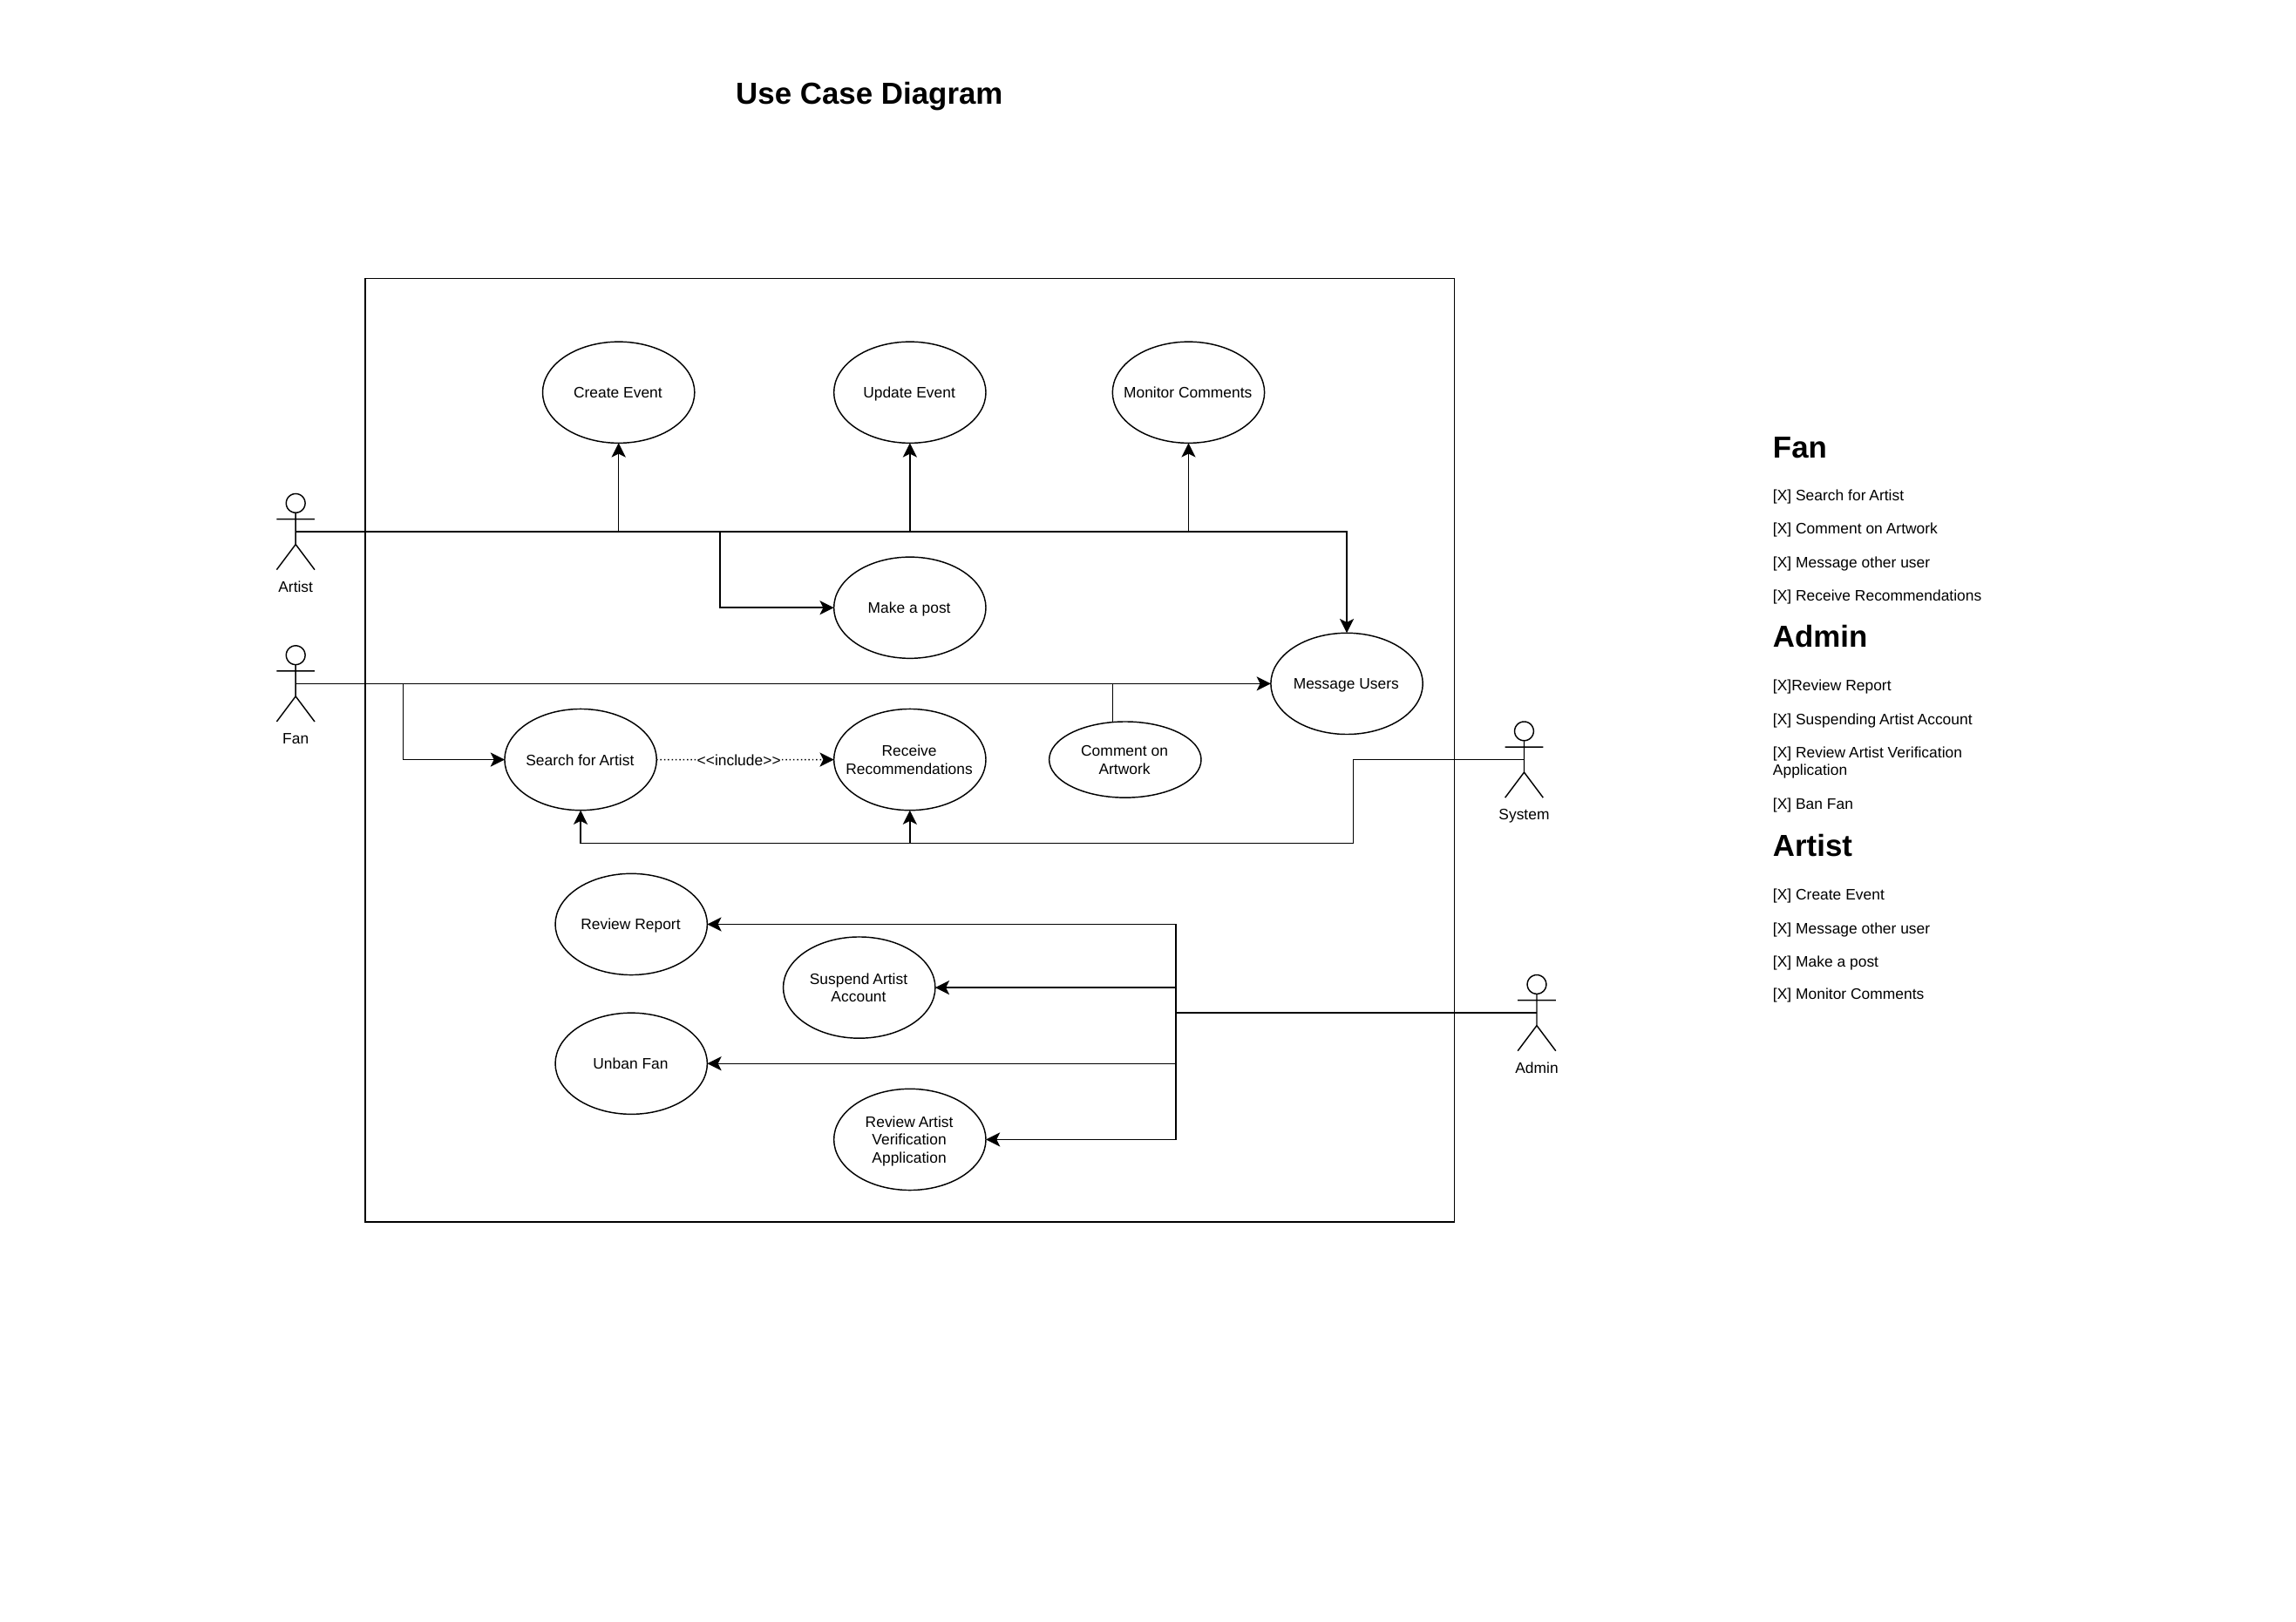
\includegraphics[width=0.7\textwidth]{../../UseCaseDiagram/UseCaseDiagram.png}
\end{frame}

% ============================================================
\section{Domain / Class Model}

\begin{frame}{Domain Model / Design Refinements}
\centering
% Example render from docs/domain-model.puml -- swap for your own model.
\fillin{Insert Domain or Class Model image here}
\end{frame}

% ============================================================
\section{Next Steps}

\begin{frame}{Looking Ahead to Iteration \nextIteration}
\begin{itemize}
  \item \fillin{Planned feature, refactoring, or bug fix for Iteration \nextIteration}
  \item \fillin{Planned feature, refactoring, or bug fix for Iteration \nextIteration}
  \item \fillin{Upcoming technical spikes or risks to address}
\end{itemize}
\end{frame}

\begin{frame}[standout]
Questions?
\end{frame}

\end{document}